\section{Strumenti forensi testati} \label{chap:strumenti}

Nel presente lavoro di tesi, è stato condotto uno studio sperimentale sulla robustezza operativa di strumenti forensi basati su Intelligenza Artificiale, con particolare riferimento alla classificazione automatica di immagini contenenti armi da fuoco. L’analisi si è focalizzata su un insieme di software e piattaforme effettivamente impiegati in ambito forense professionale, selezionati sulla base della loro diffusione, interoperabilità e capacità di supportare moduli di analisi automatizzata.

La scelta degli strumenti ha privilegiato soluzioni commerciali consolidate nel settore, in grado di operare in ambienti reali e di supportare (direttamente o indirettamente) flussi basati su tecniche di Machine Learning (ML) o Deep Learning (DL). L’obiettivo è stato quello di simulare scenari realistici di utilizzo forense e osservare il comportamento dei moduli di classificazione automatica quando esposti a perturbazioni visive di tipo \textit{adversarial} o \textit{anti-forense}.

\subsection{Magnet AXIOM}

\textbf{Magnet AXIOM} è una piattaforma di digital forensics tra le più diffuse in ambito investigativo, apprezzata per la sua capacità di estrarre e analizzare dati da fonti eterogenee come dispositivi mobili, computer, cloud e social media. AXIOM si distingue per la presenza di moduli avanzati di \textit{machine learning-assisted analysis}, impiegati per il riconoscimento automatico di contenuti sensibili, la categorizzazione di immagini e la segmentazione tematica dei dati.

Nel contesto di questa tesi, Magnet AXIOM è stato utilizzato per verificare la tenuta del modulo di classificazione automatica rispetto a immagini alterate artificialmente. Le immagini, appartenenti ai dataset descritti nei capitoli precedenti, sono state iniettate nel flusso di analisi simulando un processo standard di acquisizione e triage. Sono stati documentati i casi in cui l’algoritmo falliva la categorizzazione corretta in seguito all’applicazione di perturbazioni specifiche, evidenziando vulnerabilità simili a quelle documentate in letteratura per i modelli CNN-based esposti ad attacchi FGSM o occlusion patch~\cite{phd_unisi_068552}.


\begin{figure}[H]
    \centering
    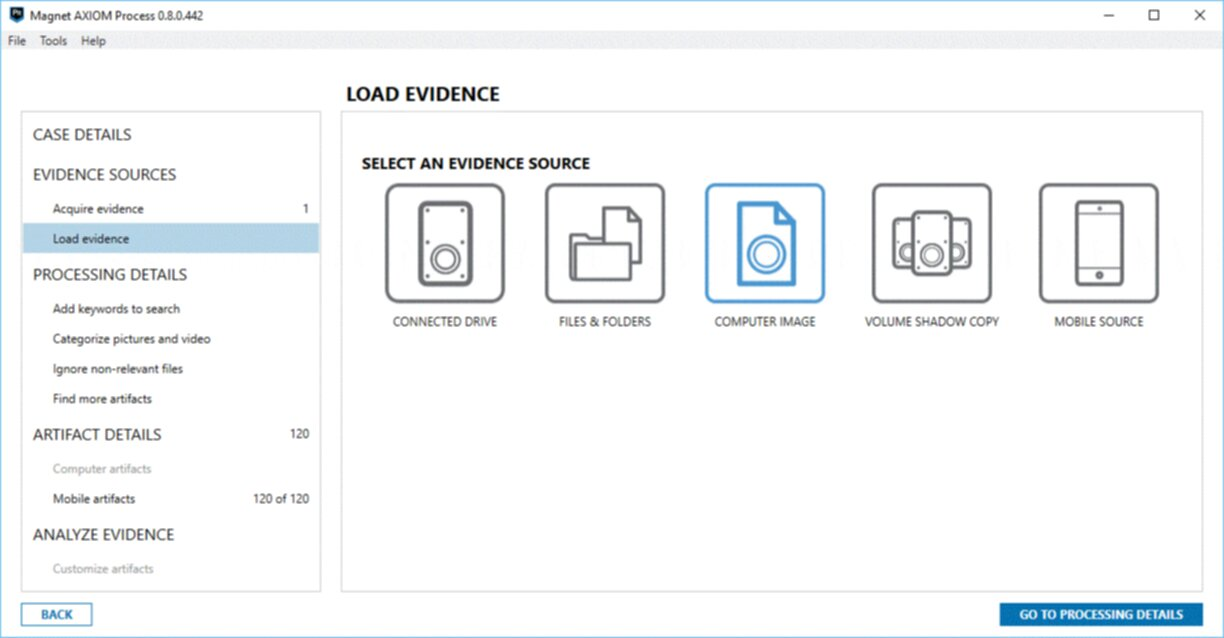
\includegraphics[width=0.75\textwidth]{images/Magnet.jpg}
    \caption{Interfaccia principale di Magnet AXIOM all'avvio del software.}
    \label{fig:magnet_axiom}
\end{figure}

\subsection{X-Ways Forensics}

\textbf{X-Ways Forensics} è uno strumento di analisi forense avanzato, noto per l’approccio \textit{low-level} all’ispezione delle immagini disco, file system e artefatti digitali. Sebbene X-Ways non implementi nativamente algoritmi di machine learning per la classificazione delle immagini, la sua architettura modulare consente l’integrazione con script esterni e moduli di analisi personalizzati. Nell’esperimento condotto, è stato sviluppato un modulo Python esterno --- basato su un modello visivo pre-addestrato (CLIP, ViT-B/32) --- integrato nel flusso di triage automatico per simulare il comportamento di una pipeline AI-based.

Questo approccio ibrido ha permesso di osservare come una soluzione legacy possa essere estesa verso scenari di classificazione automatica in ambienti forensi, pur mantenendo un alto grado di tracciabilità. Sono stati eseguiti test su immagini perturbate per verificare se le predizioni del modello integrato venissero influenzate da modifiche visive impercettibili, in linea con quanto descritto nella letteratura relativa agli attacchi adversariali applicati a contesti forensi~\cite{phd_unisi_068552, EhsanNowrooziPres}.

\begin{figure}[H]
    \centering
    \includegraphics[width=0.75\textwidth]{images/xway.png}
    \caption{Interfaccia iniziale di X-Ways Forensics con vista file system.}
    \label{fig:xways}
\end{figure}


\subsection{Cellebrite UFED}

\textbf{Cellebrite UFED (Universal Forensic Extraction Device)} è una delle soluzioni più diffuse per l’estrazione forense di dati da dispositivi mobili. Oltre alla raccolta di artefatti digitali da smartphone, tablet e SIM, UFED integra funzionalità di analisi automatizzata delle immagini, come il rilevamento di contenuti espliciti, volti o armi, mediante tecniche AI-driven.

Nella sperimentazione condotta, sono state caricate immagini selezionate e perturbate per testare la risposta del motore di classificazione visiva. I risultati hanno mostrato un degrado nella capacità del sistema di rilevare correttamente alcune classi target, con particolare evidenza nei casi di immagini sottoposte a sfocatura, compressione JPEG aggressiva o color shifting, confermando l’ipotesi che anche strumenti di fascia alta risultino vulnerabili a input avversariali~\cite{VerificationOfAI}.

\begin{figure}[H]
    \centering
    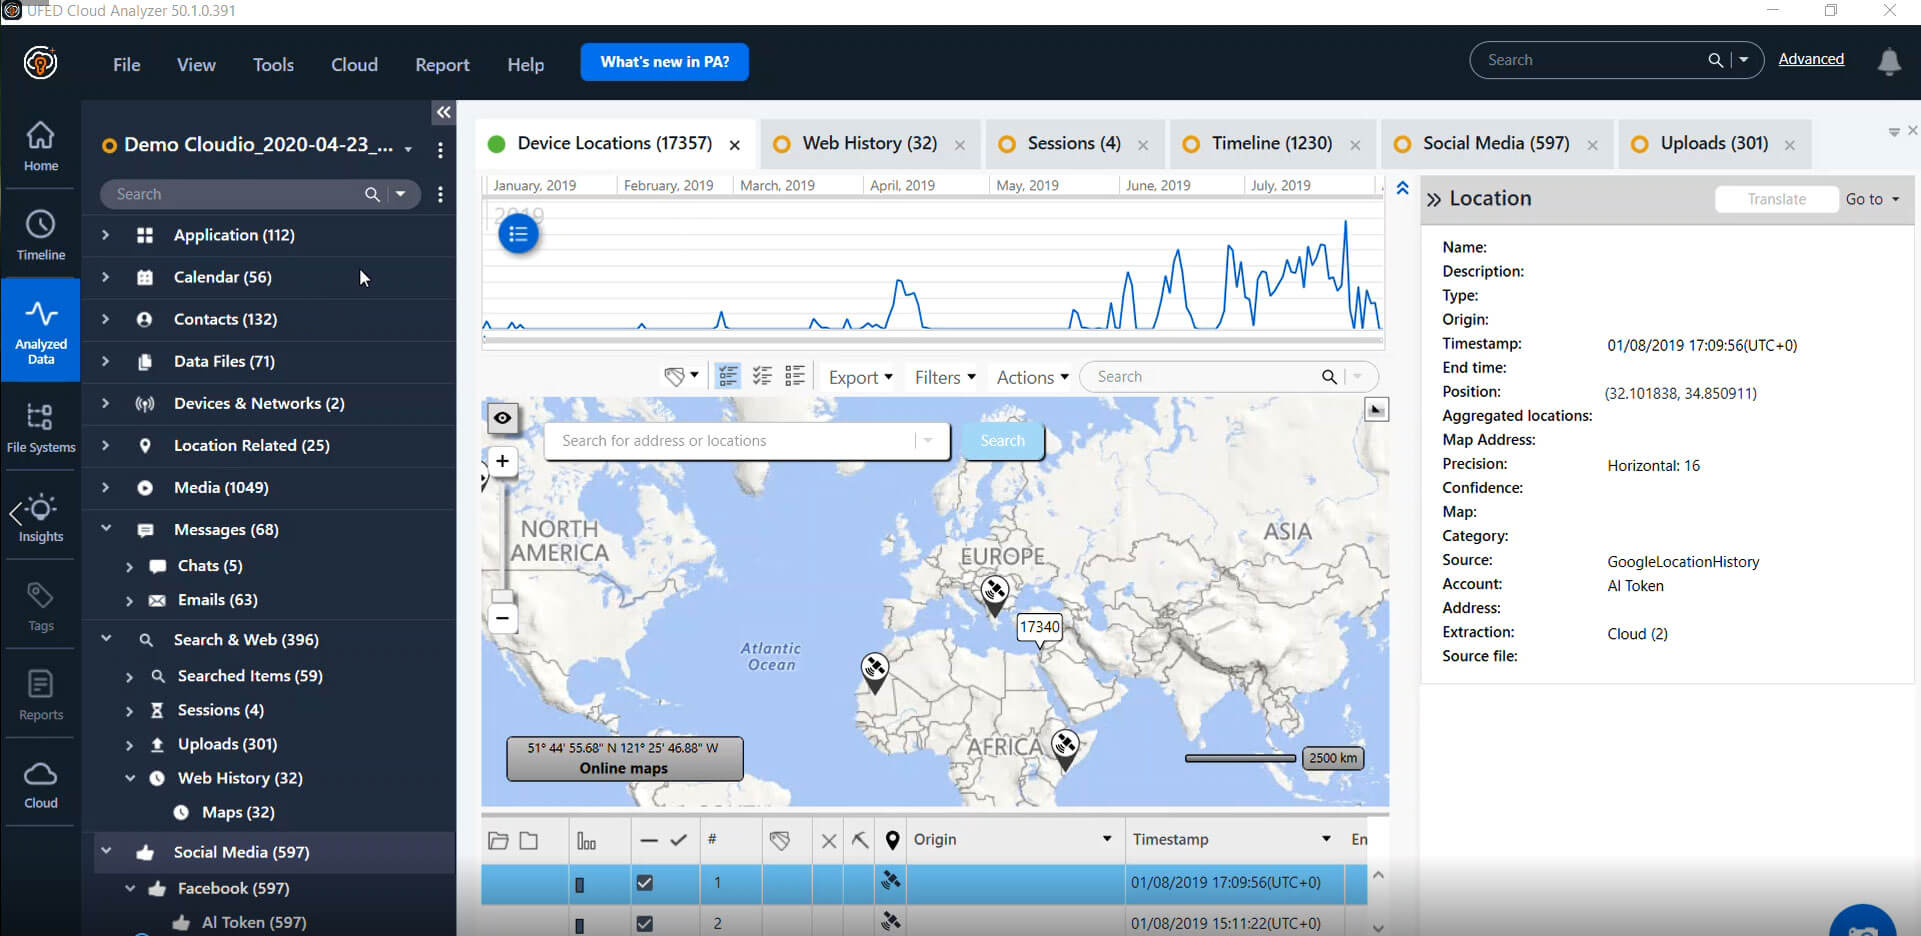
\includegraphics[width=0.75\textwidth]{images/ufed.jpg}
    \caption{Dashboard iniziale di Cellebrite UFED con riepilogo dei dispositivi acquisiti.}
    \label{fig:ufed}
\end{figure}

\subsection{Oxygen Forensics Detective}

\textbf{Oxygen Forensics Detective} è una suite forense specializzata nell’analisi di dispositivi mobili e dati cloud-based. Oltre alla raccolta di metadati e contenuti multimediali, offre funzionalità avanzate di AI per l’analisi automatica delle immagini, compresa la classificazione per contenuto, tag semantici e rilevamento di oggetti.

Sebbene le capacità di classificazione siano per lo più chiuse all’utente, è stato possibile analizzare in modalità black-box il comportamento del sistema rispetto a perturbazioni note. Le osservazioni sperimentali indicano che alcune perturbazioni visive --- in particolare quelle orientate all'occultamento di oggetti (\textit{occlusion patch}) o al mascheramento semantico --- sono in grado di ridurre significativamente la precisione del riconoscimento automatico, in linea con quanto riportato nella letteratura accademica sul tema della \textit{robustness} in AI forensics~\cite{costantini2019digital}.

\begin{figure}[H]
    \centering
    \includegraphics[width=0.75\textwidth]{images/oxygen.png}
    \caption{Vista iniziale della suite Oxygen Forensics Detective.}
    \label{fig:oxygen}
\end{figure}

\subsection{Discussione finale}

I risultati ottenuti mostrano come, pur essendo progettati per operare in contesti forensi reali, molti strumenti commerciali AI-based risultino vulnerabili a perturbazioni di natura sintetica o semantica, anche minime. Questo conferma le osservazioni riportate nella letteratura specialistica: i modelli di classificazione visiva impiegati nei tool forensi sono spesso addestrati su dataset omogenei e scarsamente esposti a variabilità realistiche o intenzionali, rendendoli suscettibili a manipolazioni mirate~\cite{phd_unisi_068552, costantini2019digital, VerificationOfAI}.

Alla luce di tali considerazioni, risulta fondamentale sviluppare metodologie di validazione che includano scenari ostili e dataset eterogenei, oltre a prevedere l’integrazione di moduli di rilevamento della manipolazione o di verifica della coerenza semantica, come illustrato nella Tabella~\ref{tab:tool-perturbazioni}.



\begin{comment}
\begin{table}[H]
\centering
\begin{tabularx}{\textwidth}{>{\raggedright\arraybackslash}p{3.5cm} >{\raggedright\arraybackslash}X >{\raggedright\arraybackslash}p{3.5cm} >{\raggedright\arraybackslash}X}
\toprule
\textbf{Strumento} & \textbf{Funzionalità AI rilevanti} & \textbf{Tipi di perturbazioni testate} & \textbf{Osservazioni sperimentali} \\
\midrule
\textbf{Magnet AXIOM} & Classificazione automatica immagini, rilevamento contenuti sensibili & FGSM, JPEG Compression, Occlusion Patch & Degradazione significativa della precisione in presenza di modifiche impercettibili o piccole occlusioni \\
\textbf{X-Ways Forensics} & Integrazione con modelli AI esterni (es. CLIP) tramite script & Color shifting, Gaussian blur, DeepFool & Vulnerabilità osservata nel modulo AI integrato, soprattutto in immagini ad alta variabilità visiva \\
\textbf{Cellebrite UFED} & Rilevamento automatico armi e contenuti sensibili in immagini da smartphone & JPEG artefacts, One Pixel Attack, Occlusion Patch & Alcune classi non rilevate correttamente in presenza di distorsioni lievi ma strategiche \\
\textbf{Oxygen Forensics Detective} & Auto-tagging semantico e categorizzazione automatica immagini & Blur, Adversarial Noise, Color Manipulation & Rilevata riduzione di precisione del riconoscimento sotto attacco visivo controllato \\
\bottomrule
\end{tabularx}
\caption{Sintesi dei tool forensi testati e del loro comportamento in presenza di perturbazioni}
\label{tab:tool-perturbazioni}
\end{table}
\end{comment}